%%%%%%%%%%%%%%%%%%%%%%%%%%%%%%%%%%%%%%%%%
% Beamer Presentation
% LaTeX Template
% Version 2.0 (March 8, 2022)
%
% This template originates from:
% https://www.LaTeXTemplates.com
%
% Author:
% Vel (vel@latextemplates.com)
%
% License:
% CC BY-NC-SA 4.0 (https://creativecommons.org/licenses/by-nc-sa/4.0/)
%
%%%%%%%%%%%%%%%%%%%%%%%%%%%%%%%%%%%%%%%%%

%----------------------------------------------------------------------------------------
%	PACKAGES AND OTHER DOCUMENT CONFIGURATIONS
%----------------------------------------------------------------------------------------
\documentclass[
	12pt, % Set the default font size, options include: 8pt, 9pt, 10pt, 11pt, 12pt, 14pt, 17pt, 20pt
	%t, % Uncomment to vertically align all slide content to the top of the slide, rather than the default centered
	aspectratio=169, % Uncomment to set the aspect ratio to a 16:9 ratio which matches the aspect ratio of 1080p and 4K screens and projectors
]{beamer}

\graphicspath{{Images/}{./}} % Specifies where to look for included images (trailing slash required)

\usepackage{booktabs} % Allows the use of \toprule, \midrule and \bottomrule for better rules in tables

%----------------------------------------------------------------------------------------
%	SELECT LAYOUT THEME
%----------------------------------------------------------------------------------------

% Beamer comes with a number of default layout themes which change the colors and layouts of slides. Below is a list of all themes available, uncomment each in turn to see what they look like.

%\usetheme{default}
%\usetheme{AnnArbor}
%\usetheme{Antibes}
%\usetheme{Bergen}
%\usetheme{Berkeley}
%\usetheme{Berlin}
\usetheme{Boadilla} %me gusta
%\usetheme{CambridgeUS}
%\usetheme{Copenhagen}
%\usetheme{Darmstadt}
%\usetheme{Dresden}
%\usetheme{Frankfurt}
%\usetheme{Goettingen} %dos dos
%\usetheme{Hannover} %dos dos
%\usetheme{Ilmenau}
%\usetheme{JuanLesPins}
%\usetheme{Luebeck}
%\usetheme{Madrid}
%\usetheme{Malmoe}
%\usetheme{Marburg}
%\usetheme{Montpellier}
%\usetheme{PaloAlto}
%\usetheme{Pittsburgh}
%\usetheme{Rochester} %muy flat
%\usetheme{Singapore}
%\usetheme{Szeged}
%\usetheme{Warsaw}

%----------------------------------------------------------------------------------------
%	SELECT COLOR THEME
%----------------------------------------------------------------------------------------

% Beamer comes with a number of color themes that can be applied to any layout theme to change its colors. Uncomment each of these in turn to see how they change the colors of your selected layout theme.

%\usecolortheme{albatross}
%\usecolortheme{beaver}
%\usecolortheme{beetle}
%\usecolortheme{crane}
%\usecolortheme{dolphin}
%\usecolortheme{dove}
%\usecolortheme{fly}
%\usecolortheme{lily} %default
%\usecolortheme{monarca}
%\usecolortheme{seagull}
%\usecolortheme{seahorse}
%\usecolortheme{spruce}
%\usecolortheme{whale}
%\usecolortheme{wolverine}

%----------------------------------------------------------------------------------------
%	SELECT FONT THEME & FONTS
%----------------------------------------------------------------------------------------

% Beamer comes with several font themes to easily change the fonts used in various parts of the presentation. Review the comments beside each one to decide if you would like to use it. Note that additional options can be specified for several of these font themes, consult the beamer documentation for more information.

\usefonttheme{default} % Typeset using the default sans serif font
%\usefonttheme{serif} % Typeset using the default serif font (make sure a sans font isn't being set as the default font if you use this option!)
%\usefonttheme{structurebold} % Typeset important structure text (titles, headlines, footlines, sidebar, etc) in bold
%\usefonttheme{structureitalicserif} % Typeset important structure text (titles, headlines, footlines, sidebar, etc) in italic serif
%\usefonttheme{structuresmallcapsserif} % Typeset important structure text (titles, headlines, footlines, sidebar, etc) in small caps serif

%------------------------------------------------

%\usepackage{mathptmx} % Use the Times font for serif text
\usepackage{palatino} % Use the Palatino font for serif text

\usepackage[ruled,vlined]{algorithm2e}
%\usepackage{helvet} % Use the Helvetica font for sans serif text
\usepackage[default]{opensans} % Use the Open Sans font for sans serif text
\usepackage[spanish]{babel}
\usepackage{dirtree}
\usepackage{xcolor}
%\usepackage[default]{FiraSans} % Use the Fira Sans font for sans serif text
%\usepackage[default]{lato} % Use the Lato font for sans serif text

\usepackage[scaled]{helvet}
\usepackage[round]{natbib}
%\newcommand{\newblock}{}

\usepackage{rotating}

\newcommand\FourQuad[4]{%
  \begin{minipage}[b][.33\textheight][t] 
    {.48\textwidth}#1\end{minipage}\hfill%
    \begin{minipage}[b][.33\textheight][t] 
      {.48\textwidth}#2\end{minipage}\\[0.5em]
      \begin{minipage}[b][.33\textheight][t] 
        {.48\textwidth}#3\end{minipage}\hfill
        \begin{minipage}[b][.33\textheight][t] 
          {.48\textwidth}#4\end{minipage}%
}

\usepackage{tikz}
%\usetikzlibrary{arrows,shapes,positioning,shadows,trees,quotes}


%\tikzset{
%  basic/.style  = {draw, text width=2cm, drop shadow, font=\sffamily, rectangle},
%  root/.style   = {basic, rounded corners=2pt, thin, align=center,
%                   fill=green!30},
%  level 2/.style = {basic, rounded corners=6pt, thin,align=center, fill=green!60,
%                   text width=8em},
%  level 3/.style = {basic, thin, align=left, fill=pink!60, text width=6.5em}
%}

\usetikzlibrary{calc}

\tikzstyle{part} = [rectangle, rounded corners, minimum width=3cm, minimum height=1cm,     align=center, draw=black]
\tikzstyle{chapter} = [rectangle, rounded corners, minimum width=3cm, minimum height=1cm,     align=center, draw=black, text width=3.5cm]
\tikzstyle{arrow} = [thick, ->]

\usepackage{array} % needed for \arraybackslash
\usepackage{graphicx}
\usepackage{adjustbox} % for \adjincludegraphics

\usepackage{subcaption}
\usepackage{bibentry}
%\bibliographystyle{apalike}
\usepackage{chngcntr}
\usepackage{lipsum}% http://ctan.org/pkg/lipsum
\usepackage{hanging}% http://ctan.org/pkg/hanging

\usepackage{xcolor,colortbl}
\usepackage{multirow}

\usepackage{animate}
\usepackage{multicol}
\usepackage{tabularx,booktabs}
\usepackage{forloop}
\usepackage{ragged2e}

\usepackage{bbding} %palomitas checkmark
\usepackage{pifont}

\newcounter{loopcntr}
%----------------------------------------------------------------------------------------
%	SELECT INNER THEME
%----------------------------------------------------------------------------------------

% Inner themes change the styling of internal slide elements, for example: bullet points, blocks, bibliography entries, title pages, theorems, etc. Uncomment each theme in turn to see what changes it makes to your presentation.

%\useinnertheme{default}
\useinnertheme{circles}
%\useinnertheme{rectangles}
%\useinnertheme{rounded}
%\useinnertheme{inmargin}

%----------------------------------------------------------------------------------------
%	SELECT OUTER THEME
%----------------------------------------------------------------------------------------

% Outer themes change the overall layout of slides, such as: header and footer lines, sidebars and slide titles. Uncomment each theme in turn to see what changes it makes to your presentation.

%\useoutertheme{default}
%\useoutertheme{infolines}
%\useoutertheme{miniframes}
%\useoutertheme{smoothbars}
%\useoutertheme{sidebar}
%\useoutertheme{split}
%\useoutertheme{shadow}
%\useoutertheme{tree}
%\useoutertheme{smoothtree}

%\setbeamertemplate{footline} % Uncomment this line to remove the footer line in all slides
\setbeamertemplate{footline}[page number] % Uncomment this line to replace the footer line in all slides with a simple slide count
%\setbeamertemplate{caption}[numbered]
\setbeamertemplate{navigation symbols}{} % Uncomment this line to remove the navigation symbols from the bottom of all slides

%----------------------------------------------------------------------------------------
%	PRESENTATION INFORMATION
%----------------------------------------------------------------------------------------

\title[PROTOCOLO DE INVESTIGACIÓN]{%\centering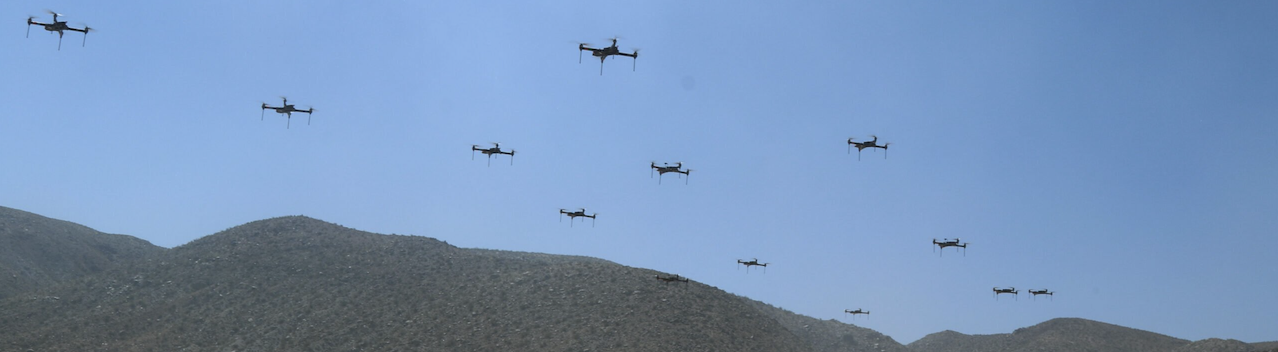
\includegraphics[width=10cm]{swarm_drones}\\
  Estrategias para la exploración coordinada multi-VANT} % The short title in the optional parameter appears at the bottom of every slide, the full title in the main parameter is only on the title page

%\subtitle{Optional Subtitle} % Presentation subtitle, remove this command if a subtitle isn't required

\author[Luis Ballado]{Luis Alberto Ballado Aradias} % Presenter name(s), the optional parameter can contain a shortened version to appear on the bottom of every slide, while the main parameter will appear on the title slide

\institute[CINVESTAV]{
  CINVESTAV UNIDAD TAMAULIPAS \\
  %\smallskip \textit{luis.ballado@cinvestav.mx}
} % Your institution, the optional parameter can be used for the institution shorthand and will appear on the bottom of every slide after author names, while the required parameter is used on the title slide and can include your email address or additional information on separate lines

\date[\today]{Cd. Victoria, Tamaulipas - \today} % Presentation date or conference/meeting name, the optional parameter can contain a shortened version to appear on the bottom of every slide, while the required parameter value is output to the title slide

%\titlegraphic{\hspace*{8.75cm}~%
%   
\includegraphics[width=0.8cm]{cinvestavlogo}
%}

%----------------------------------------------------------------------------------------

\counterwithin*{footnote}{page}
\newcommand\footcite[1]{\footnote{\bibentry{#1}}\label{\thepage:#1}}
\newcommand\secondcite[1]{\textsuperscript{\ref{\thepage:#1}}}

\newcommand{\rpt}[2][1]{%
  \forloop{loopcntr}{0}{\value{loopcntr}<#1}{#2}%
}
\newcommand{\on}[1][1]{
  \forloop{loopcntr}{0}{\value{loopcntr}<#1}{&\cellcolor{gray}}
}
\newcommand{\off}[1][1]{
  \forloop{loopcntr}{0}{\value{loopcntr}<#1}{&}
}

\addtolength{\textheight}{90pt}

\newcommand{\I}{\mathbb{I}}
\newcommand{\K}{\mathbb{K}}
\newcommand{\N}{\mathbb{N}}
\newcommand{\Q}{\mathbb{Q}}
\newcommand{\R}{\mathbb{R}}
\newcommand{\Z}{\mathbb{Z}}

\newcommand{\specialcell}[2][c]{%
  \begin{tabular}[#1]{@{}c@{}}#2\end{tabular}}


\begin{document}

%----------------------------------------------------------------------------------------
%	TITLE SLIDE
%----------------------------------------------------------------------------------------

\begin{frame}
  \titlepage % Output the title slide, automatically created using the text entered in the PRESENTATION INFORMATION block above
\end{frame}

%----------------------------------------------------------------------------------------
%	TABLE OF CONTENTS SLIDE
%----------------------------------------------------------------------------------------

% The table of contents outputs the sections and subsections that appear in your presentation, specified with the standard \section and \subsection commands. You may either display all sections and subsections on one slide with \tableofcontents, or display each section at a time on subsequent slides with \tableofcontents[pausesections]. The latter is useful if you want to step through each section and mention what you will discuss.
\AtBeginSection[]
{
  \begin{frame}
    \frametitle{Contenido} % Slide title, remove this command for no title
    \tableofcontents[currentsection] % Output the table of contents (all sections on one slide)
    %\tableofcontents[pausesections] % Output the table of contents (break sections up across separate slides)
  \end{frame}
}
%----------------------------------------------------------------------------------------
%	PRESENTATION BODY SLIDES
%----------------------------------------------------------------------------------------

%\section{Introducción} % Sections are added in order to organize your presentation into discrete blocks, all sections and subsections are automatically output to the table of contents as an overview of the talk but NOT output in the presentation as separate slides

%------------------------------------------------

% Ejemplo imagen
%\begin{figure}
%  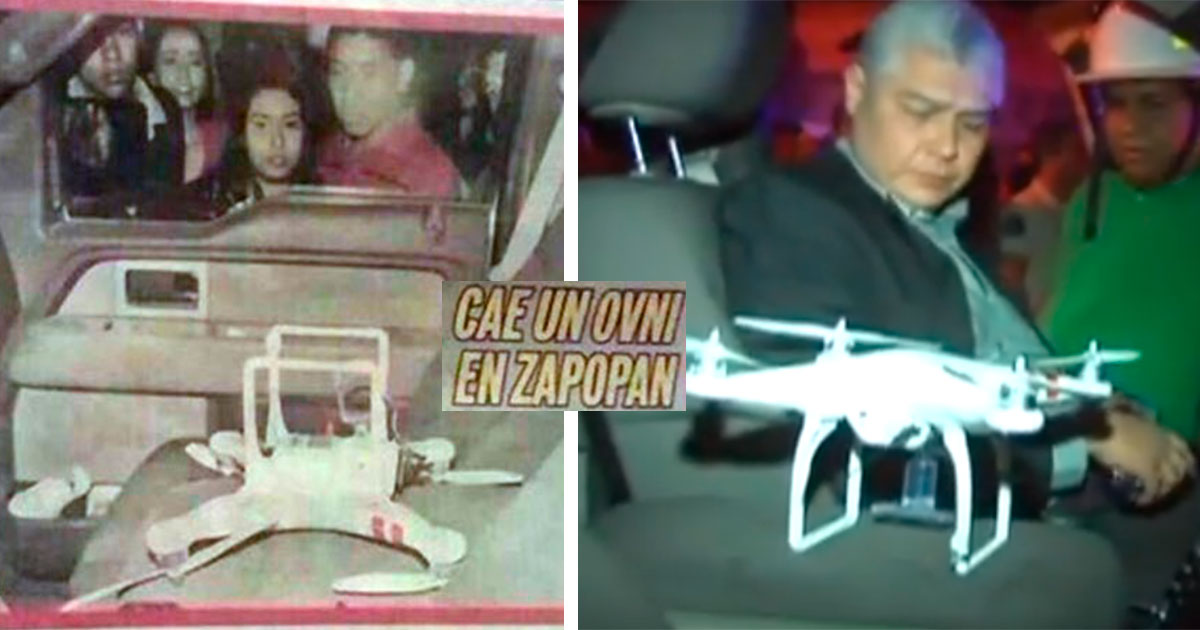
\includegraphics[width=0.7\linewidth]{dron_ovni.jpg}
%\end{figure}

\section{Resumen}

\begin{frame}{Problemática}
  %Desastres Naturales \ref{fig:images} Terremoto Turquía y norte de Siria Febrero 2023, \ref{fig:nature1} and \ref{fig:nature2}, that I can reference independently.

  %\begin{figure}
  %  \centering
  %  \begin{subfigure}[t]{0.4\textwidth}
  %    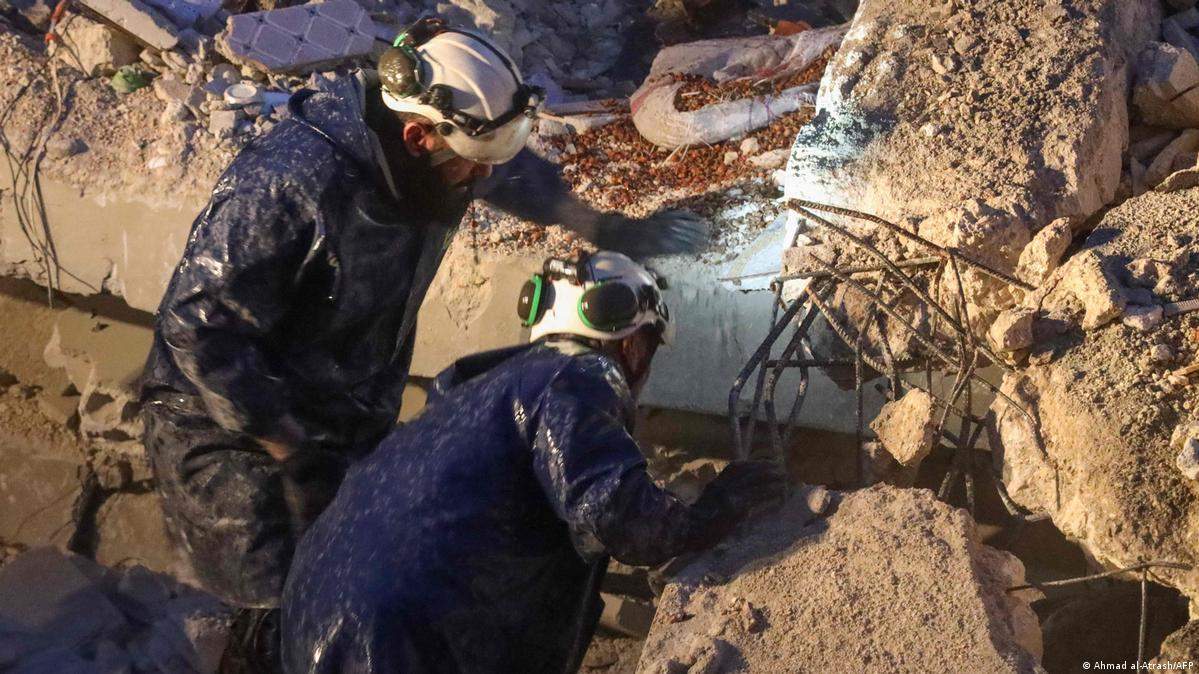
\includegraphics[width=\textwidth]{turquia1}
  %    \caption{Trabajos contra reloj en búsqueda de sobrevivientes.}
  %    \label{fig:nature1}
  %  \end{subfigure}
  %  \begin{subfigure}[b]{0.5\textwidth}
  %    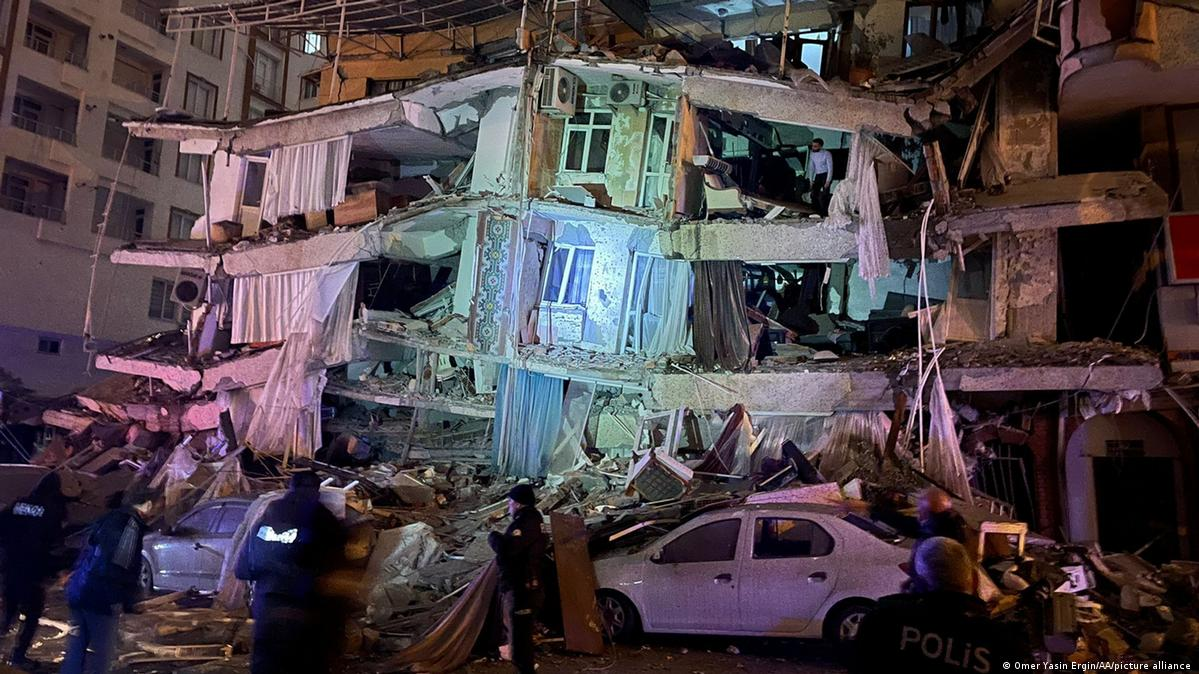
\includegraphics[width=\textwidth]{turquia2}
  %    \caption{Desastre ocurrido 4:17 am. de un Lunes por la mañana según medios internacionales.}
  %    \label{fig:nature2}
  %  \end{subfigure}
  %  \caption{Terremoto Turquía y norte de Siria Febrero 2023.}
  %  \label{fig:images}
  %\end{figure}

  \centering
  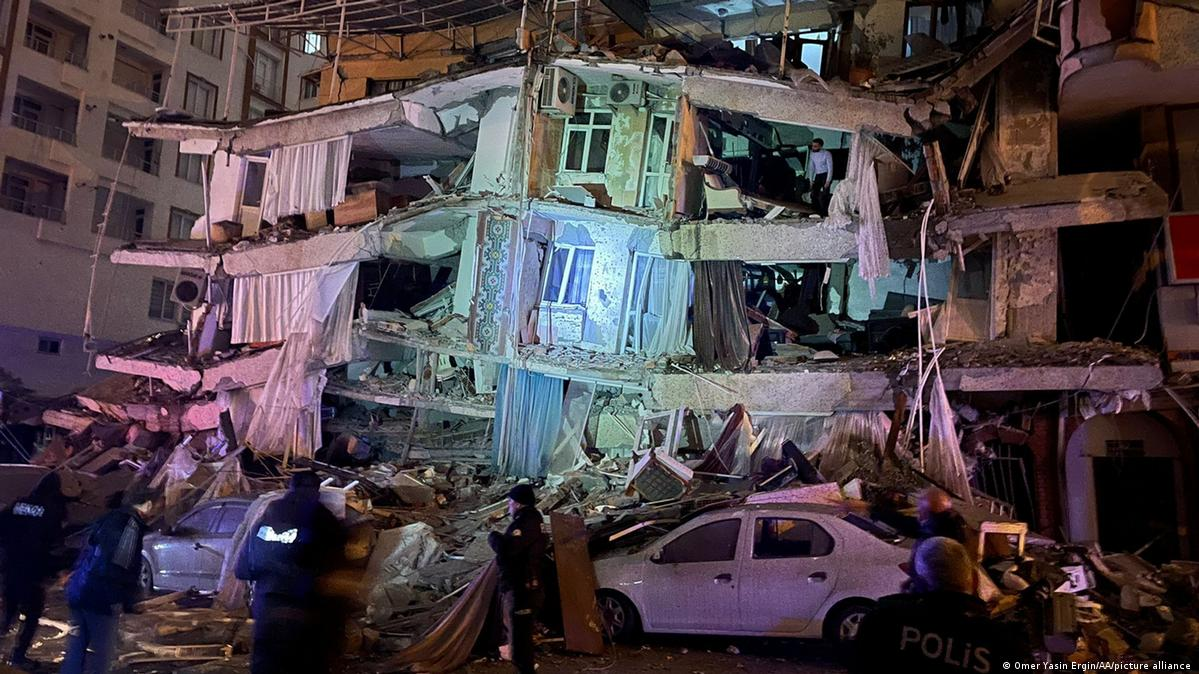
\includegraphics[width=0.45\textwidth,height=0.35\textheight]{turquia2}
  %\hfil
  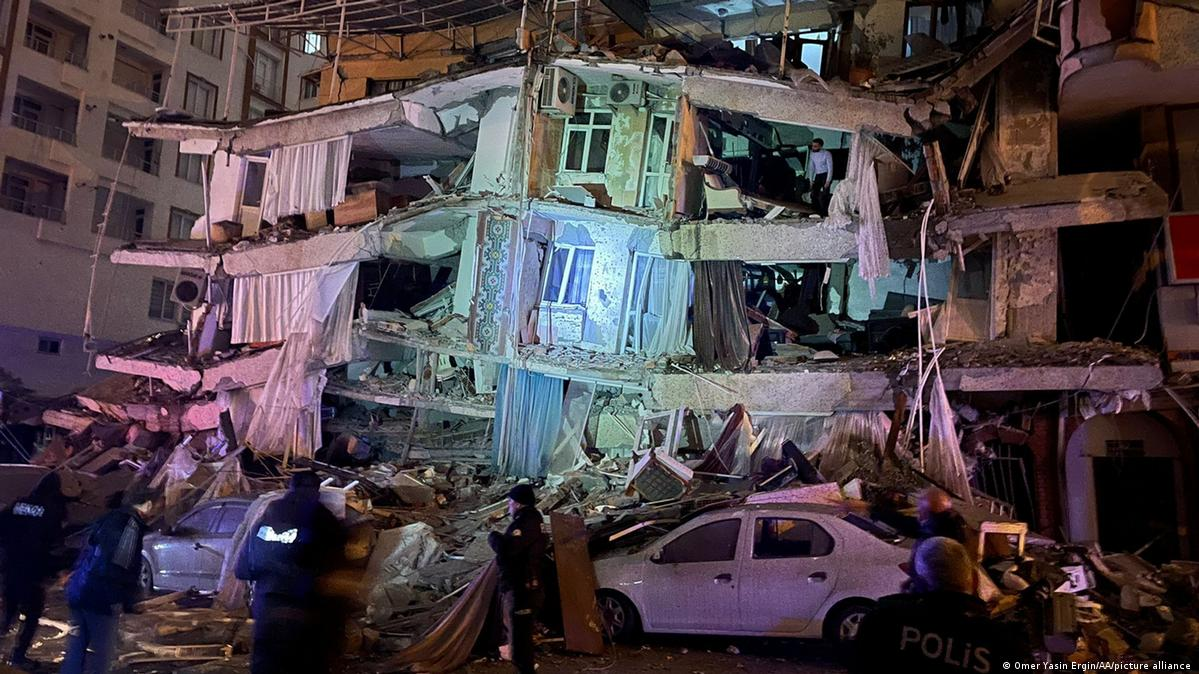
\includegraphics[width=0.45\textwidth,height=0.35\textheight]{turquia2}
  %\vspace{9pt}
  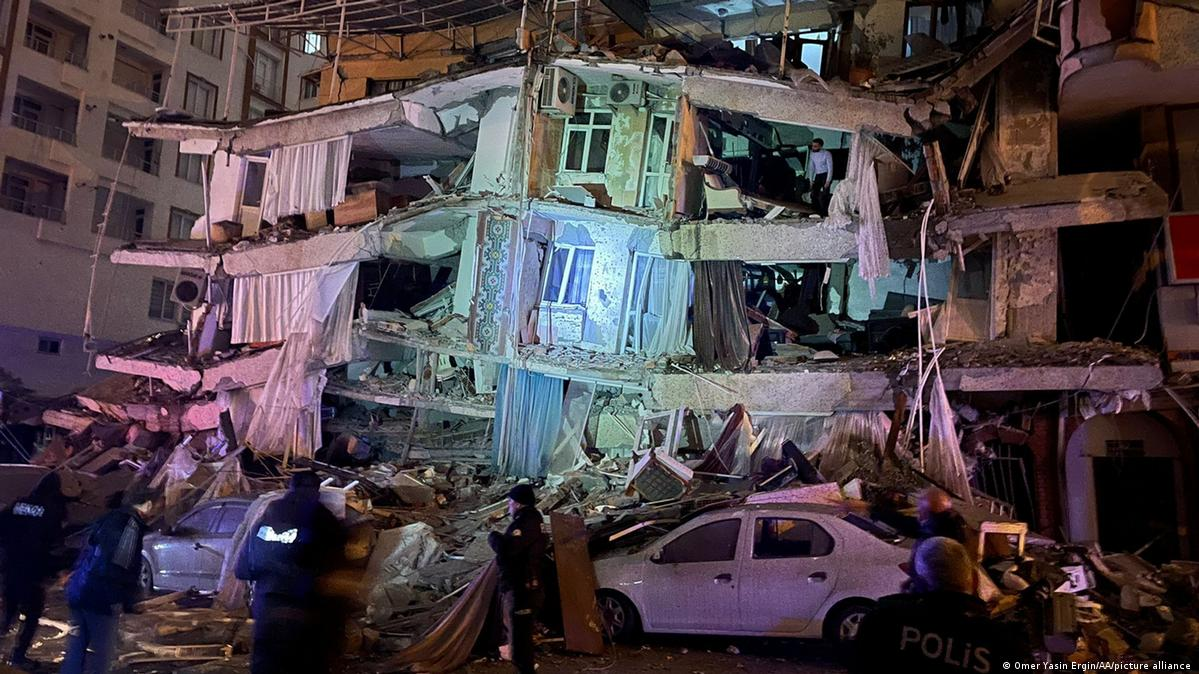
\includegraphics[width=0.45\textwidth,height=0.35\textheight]{turquia2}
  %\hfil
  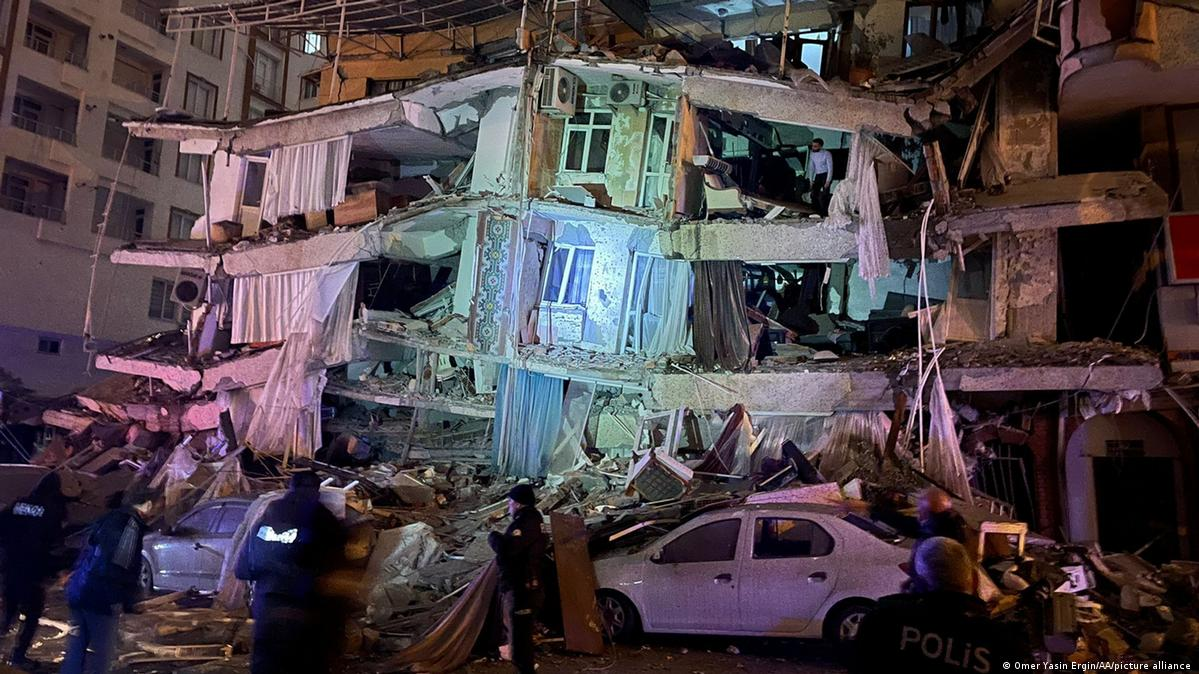
\includegraphics[width=0.45\textwidth,height=0.35\textheight]{turquia2}
  \captionof{figure}{Nice overview! Let's look get into more detail on each image.}
\end{frame}

\section{Descripción del proyecto}

\begin{frame}{Descripción del proyecto}
  \begin{minipage}{0.47\textwidth}
    \begin{itemize}
    \item<1-> First item
    \item<2-> Second item
    \item<3-> Third item
    \item<4-> Four
    \item<5-> Five
    \end{itemize}
  \end{minipage}
  \begin{minipage}{0.5\textwidth}
    \only<1>{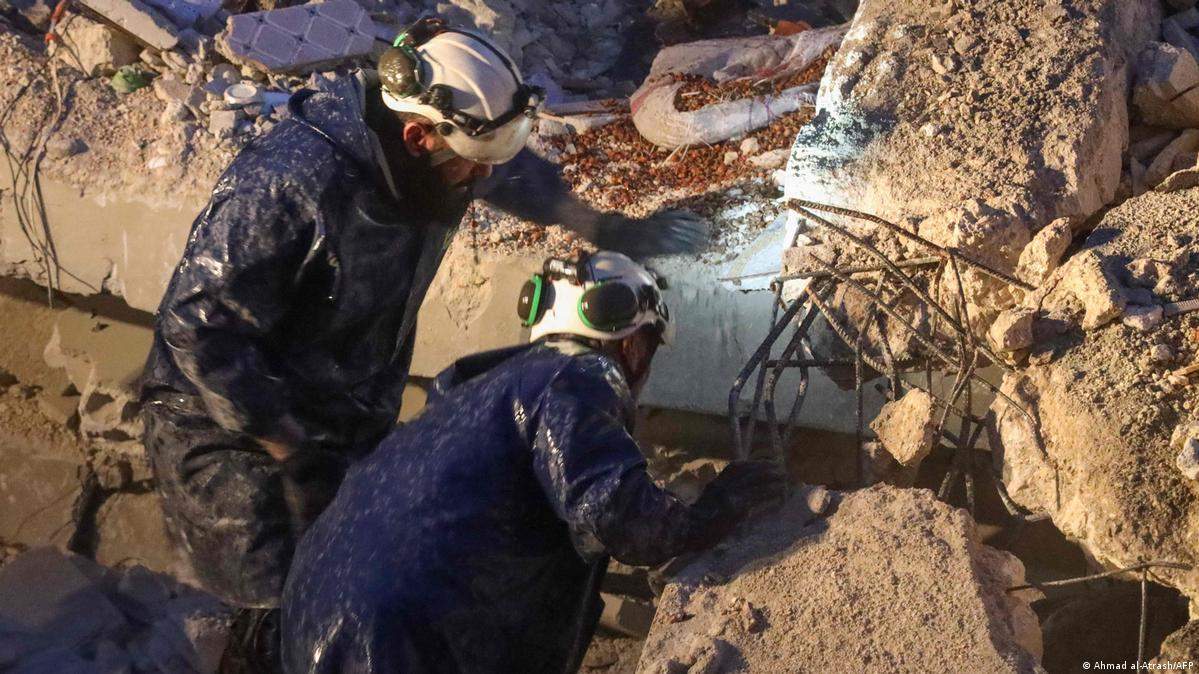
\includegraphics[width=\textwidth]{turquia1}}
    \only<2>{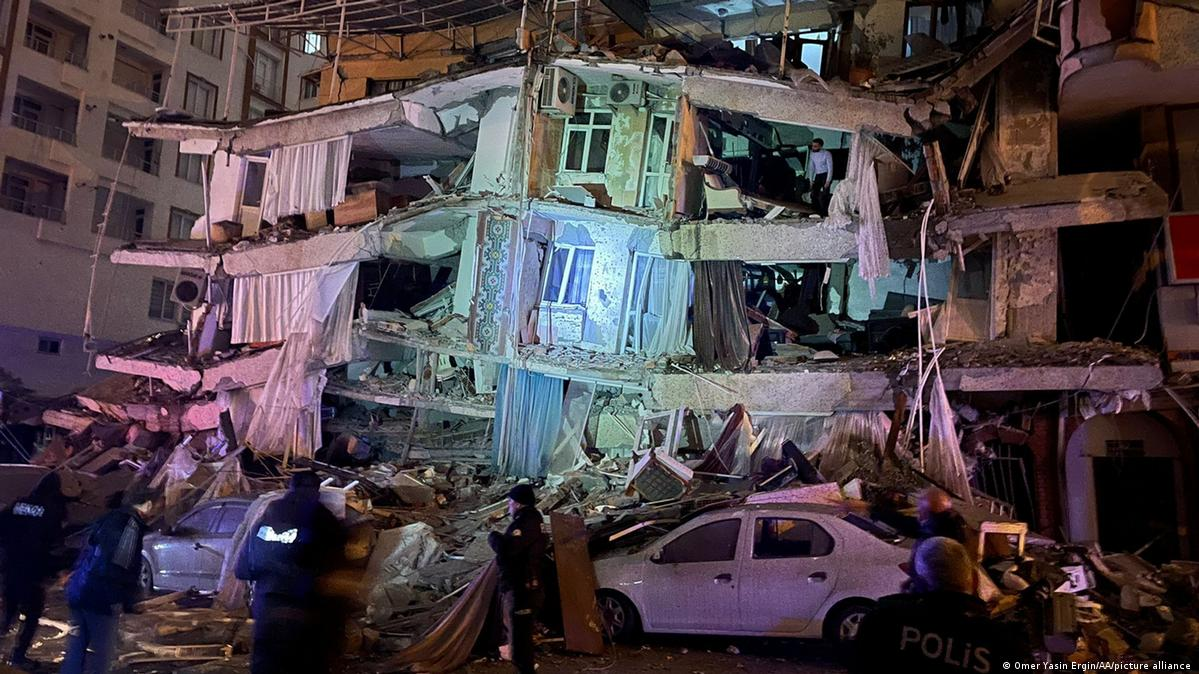
\includegraphics[width=\textwidth]{turquia2}}
    \only<3>{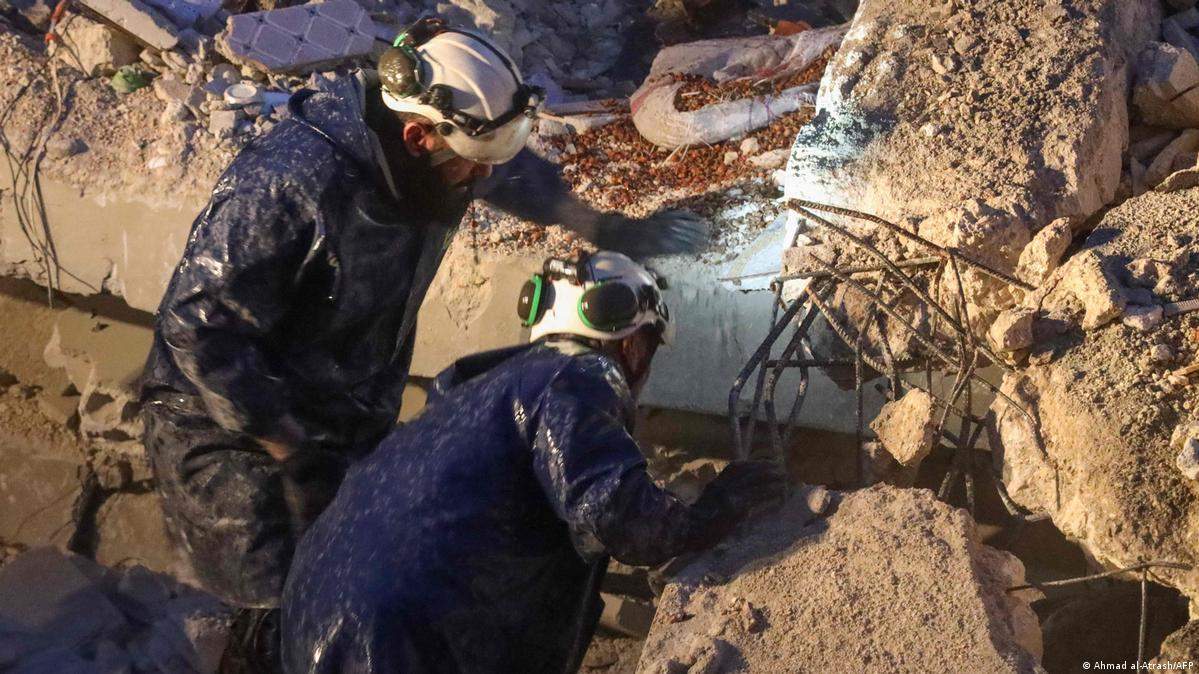
\includegraphics[width=\textwidth]{turquia1}}
    \only<4>{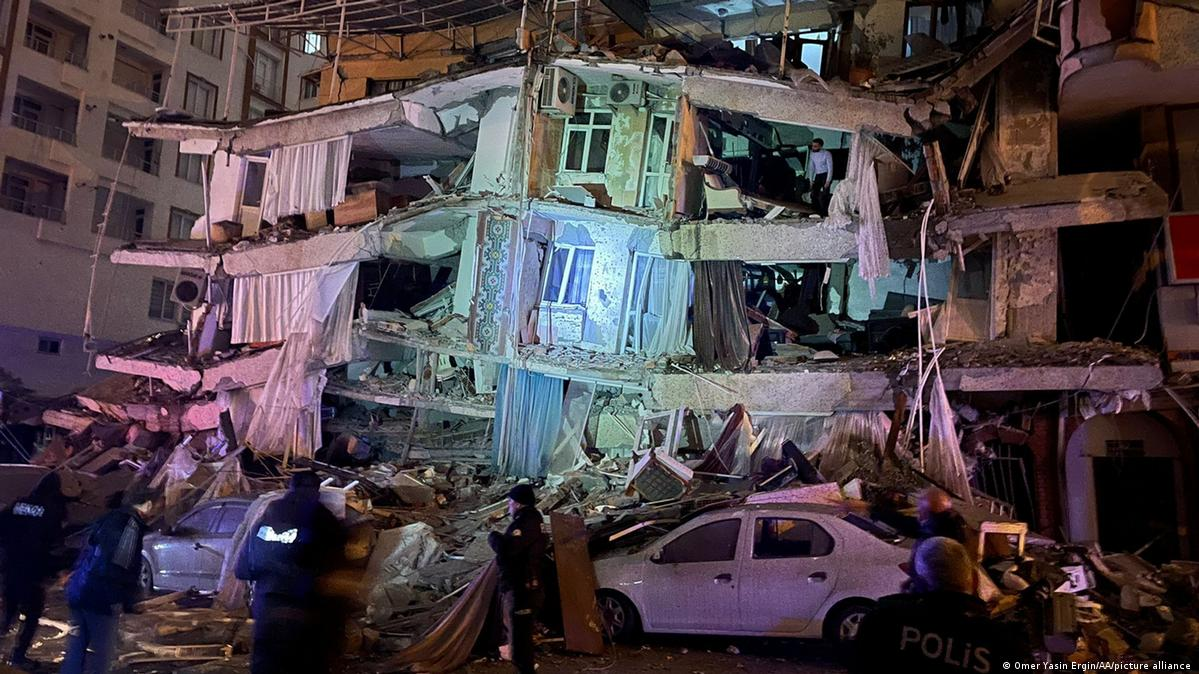
\includegraphics[width=\textwidth]{turquia2}}
    \only<5>{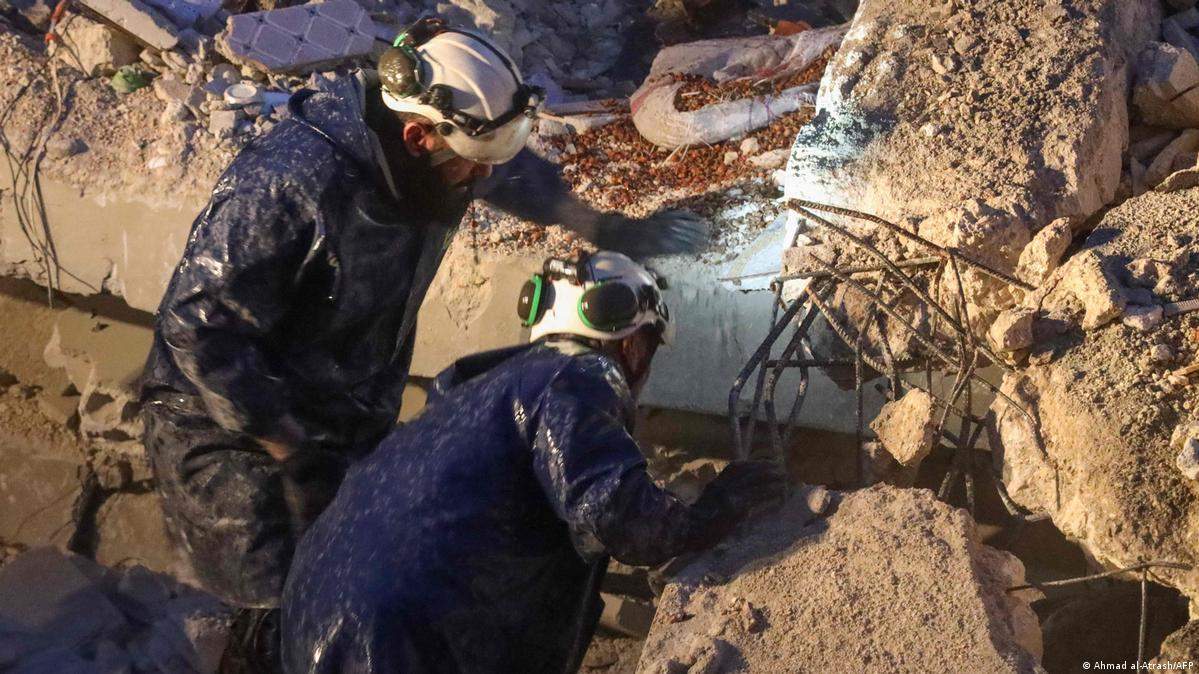
\includegraphics[width=\textwidth]{turquia1}}
  \end{minipage}
\end{frame}

\section{Antecedentes y motivación para el proyecto}
\begin{frame}{Arquitectura híbrida}
  \begin{figure}
    \centering
    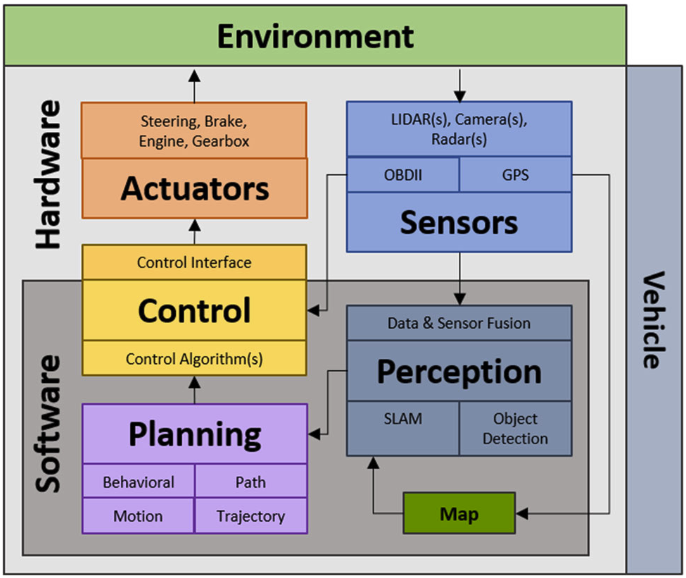
\includegraphics[scale=0.30]{control_autonomo2}$^\dag$\\
    \rule{0in}{1.2em}$^\dag$\scriptsize Hardware in the loop framework proposal for a semi-autonomous car architecture in a closed route environment \cite{CurielRamirez2019}\\
    
  \end{figure}
  %\footnotetext{Hardware in the loop framework proposal for a semi-autonomous car architecture in a closed route environment \cite{CurielRamirez2019}}
\end{frame}

\begin{frame}{Multi-robots}
  \begin{columns}
    \column{0.5\textwidth}
    Beneficios coordinación multi-VANT
    \begin{itemize}
    \item Eficiencia y cobertura
    \item Redundancia y tolerancia a fallos
    \item Adaptabilidad a entornos dinámicos
    \item Distribución de carga de trabajo
    \item Aprendizaje colaborativo
    \end{itemize}
    \column{0.5\textwidth}
    Retos multi-VANT
    \begin{itemize}
    \item Eficiencia y cobertura
    \item Redundancia y tolerancia a fallos
    \item Adaptabilidad a entornos dinámicos
    \item Distribución de carga de trabajo
    \item Aprendizaje colaborativo
    \end{itemize}
  \end{columns}
\end{frame}

%COMPARACION DE METODOS, USAR INFOGRAFIA

%\begin{frame}{}
%  \centering
%  \begin{tabular}{ |p{1.5cm}||p{0.8cm}|p{0.8cm}|p{1.2cm}|p{5cm}|  }
%    \hline
%    \multicolumn{5}{|c|}{\tiny Comparaci\'{o}n de m\'{e}todos} \\
%    \hline 
%    \tiny Metodo& \tiny Completo & \tiny \'{O}ptimo& \tiny Escalable& \tiny Notas \\
%    \hline
%    \tiny Grafo de Visibilidad   & \tiny Si    & \tiny Si&   \tiny No& \tiny Poca escalabilidad, el robot pasa cerca de los obstaculos\\
%    \hline
%    \tiny Diagramas de Voronoi   & \tiny Si    & \tiny No&   \tiny No& \tiny Poca escalabilidad\\
%    \hline
%    \tiny Campo de potencial artificial & \tiny Si    & \tiny No&   \tiny Depende del ambiente& \tiny F\'{a}cil de implementar, suceptible a minimos locales\\
%    \hline
%    \tiny Dijkstra/A*/D* & \tiny Si    & \tiny Grafo&   \tiny No& \tiny A* usa una función heuristica que guía la búsqueda más eficiente, Poca escalabilidad\\
%    \hline
%    \tiny PRM   & \tiny Si    & \tiny Grafo&   \tiny Si&  \tiny Eficiente para multi-busquedas, completez probabilistica \\
%    \hline
%    \tiny RRT   & \tiny Si    & \tiny No&   \tiny Si&  \tiny Eficiente para problemas simples, completez probabilistica\\
%    \hline
%  \end{tabular}  
%\end{frame}


\begin{frame}{Panorama Planificación de trayectorias}
  %\cite{nphard}[\citenum{nphard}] \cite{5427034}[\citenum{5427034}]
  %Calcular la ruta más corta entre dos puntos en un ambiente 3D es un problema NP-HARD.
  %La mayoria de planificadores de rutas hacen uso de heuristicas y metaheuristicas para
  %generar el óptimo más cercano \\
  \begin{figure}
    \centering
    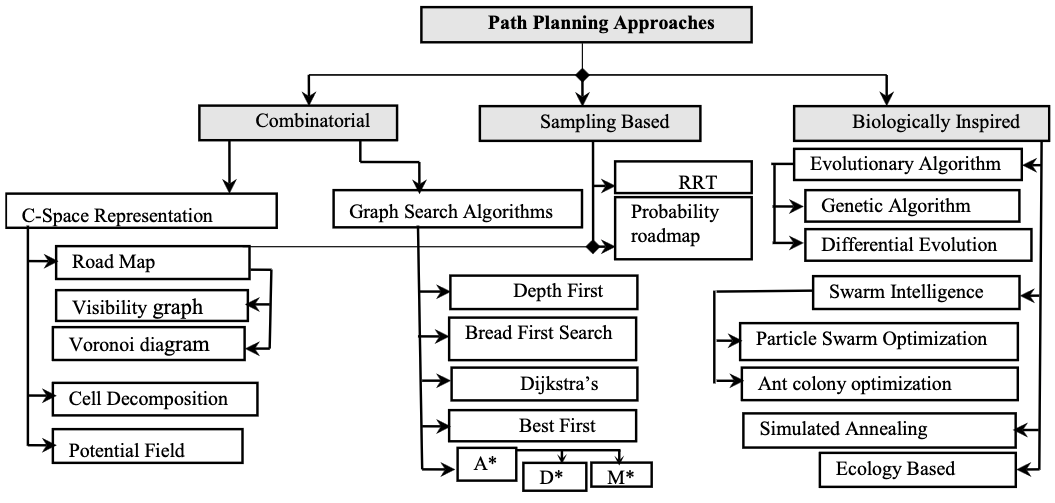
\includegraphics[scale=0.33]{path_planning_panorama}
    \caption[Caption for LOF]{Clasificación del enfoque de planificación de rutas\footnotemark}
  \end{figure}
  \footnotetext{Different Cell Decomposition Path Planning Methods for Unmanned Air Vehicles - A Review \cite{Debnath2020}}
  
\end{frame}

\begin{frame}{Representación del ambiente}
  %MOSTRAR OCTOMAP
  %MOSTRAR MAPA 3D
  \begin{figure}
    \centering
    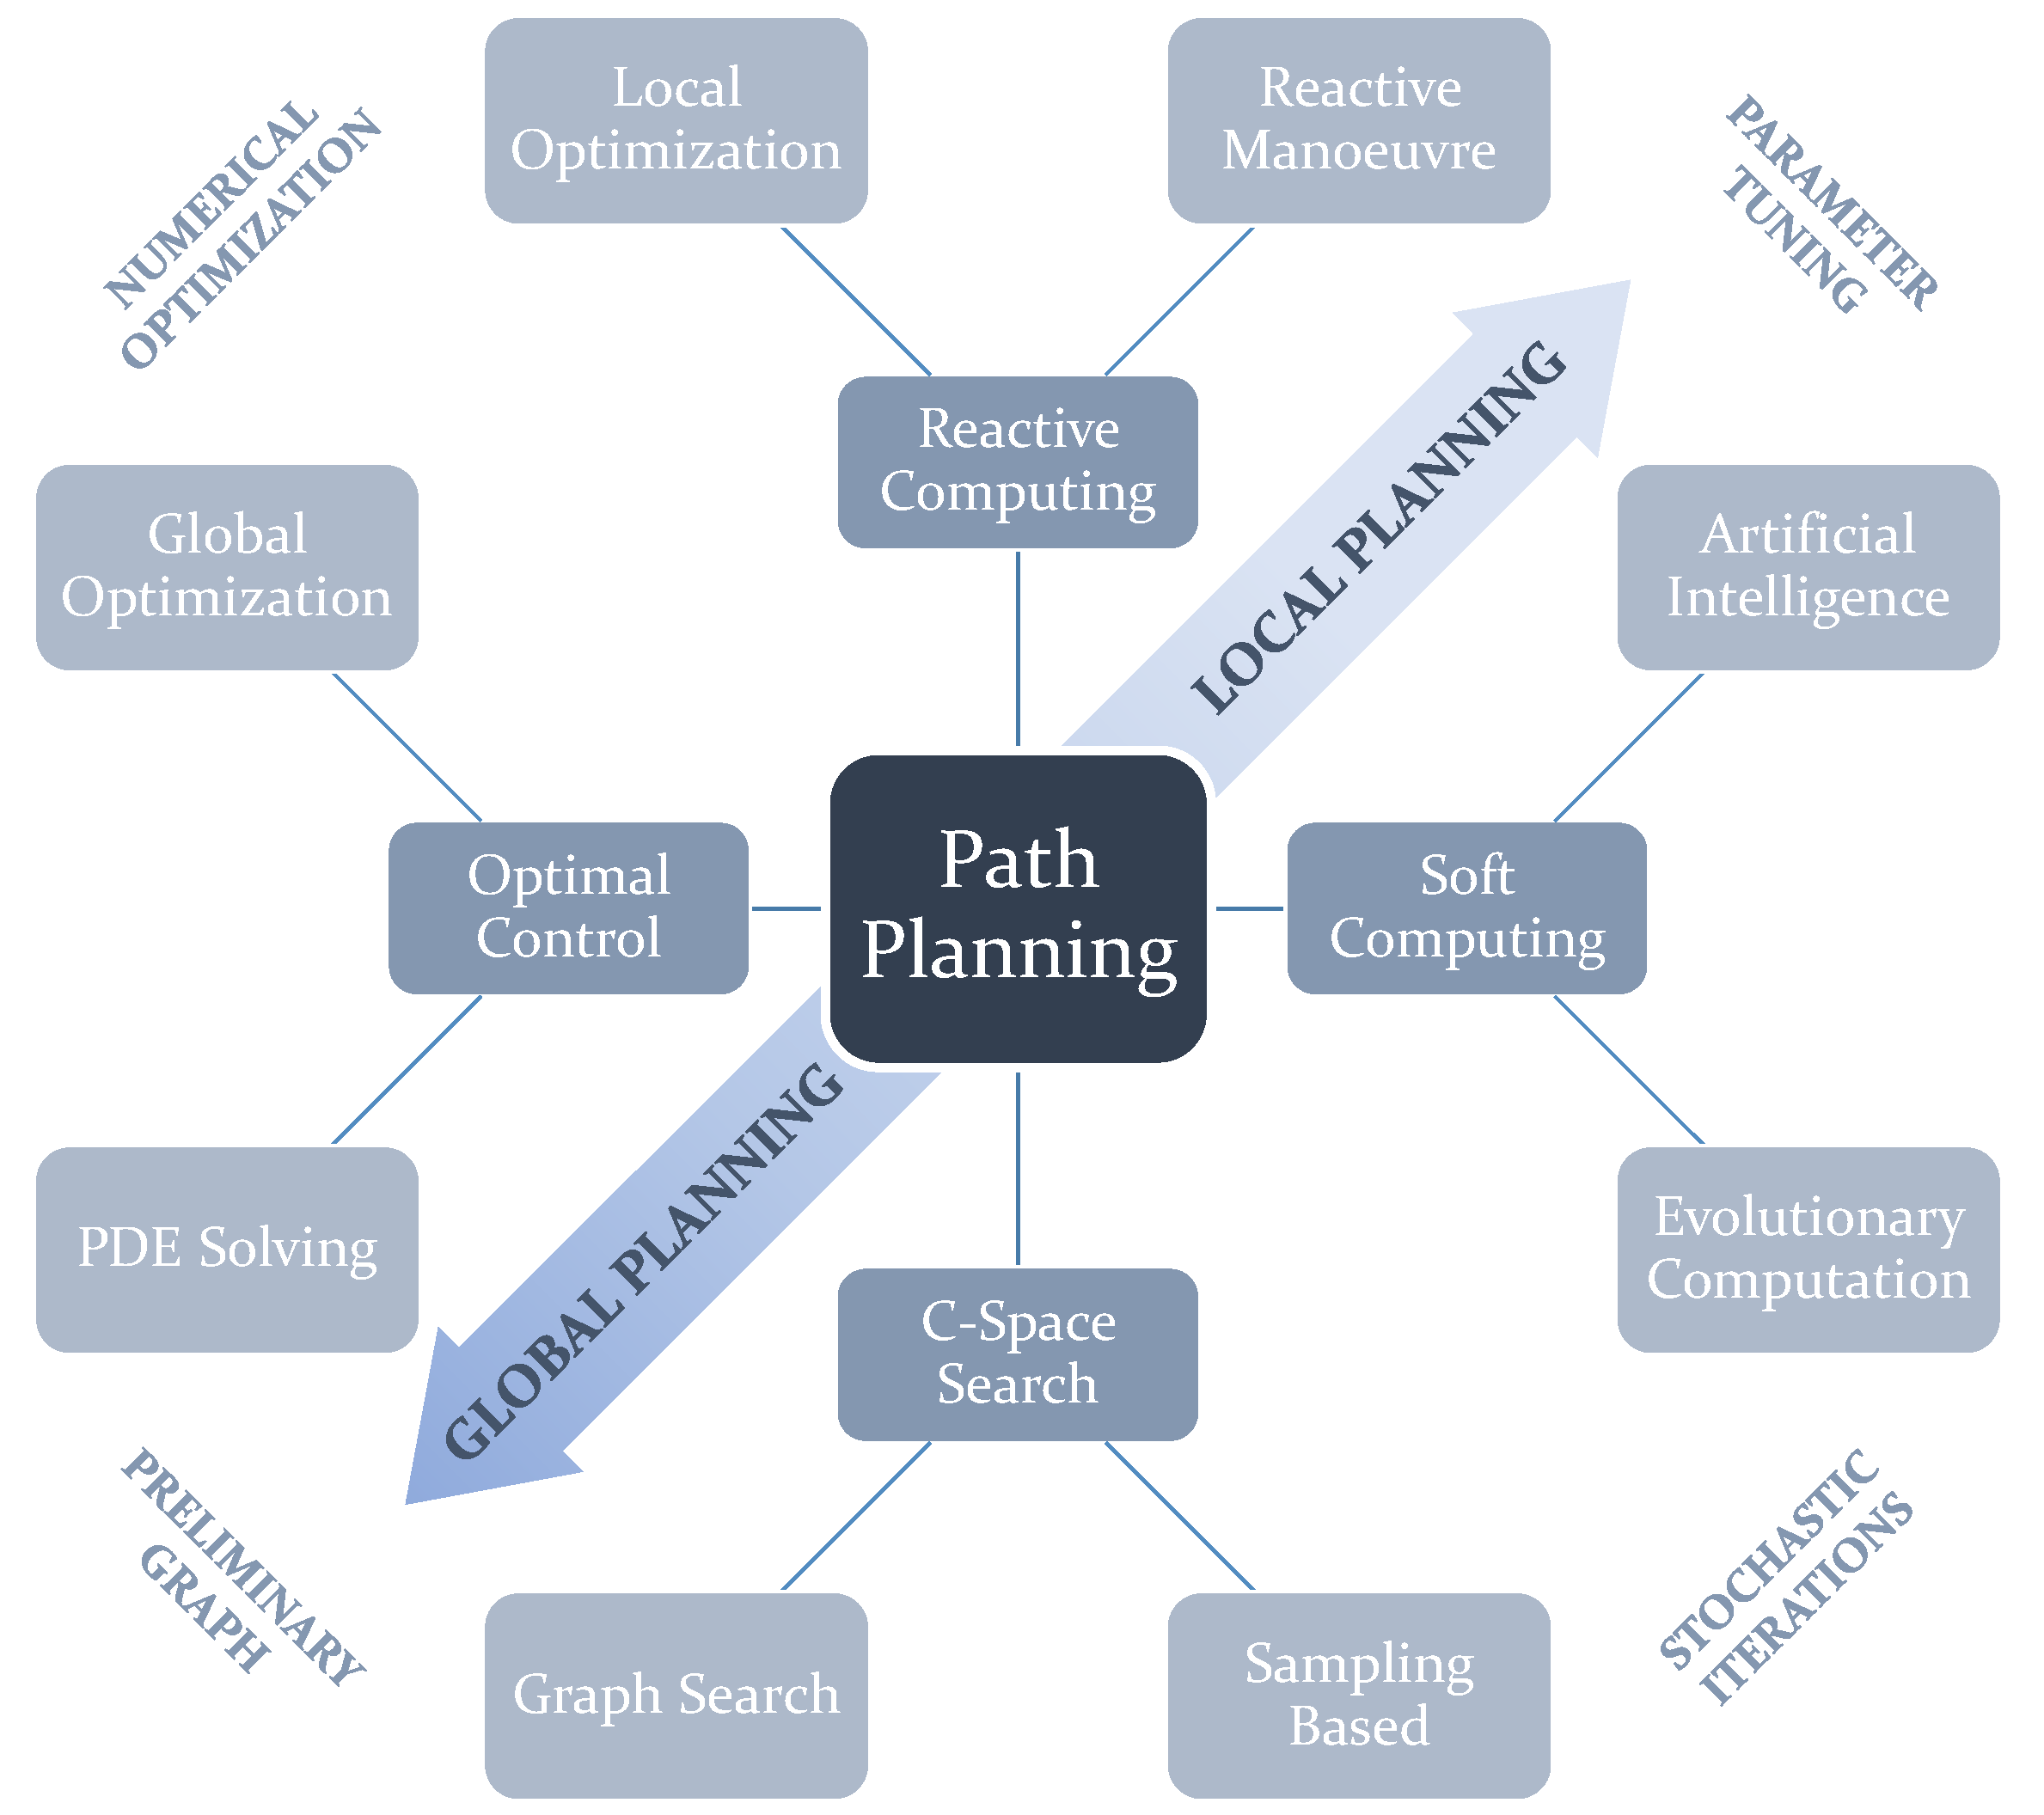
\includegraphics[scale=0.60]{panorama_planning}
    \caption[Caption for LOF]{Mapa probabilistico 3D\protect\footnotemark}
  \end{figure}
  \footnotetext{Cooperación en robots heterogeneos}
  
\end{frame}

\section{Planteamiento del problema}

\begin{frame}
  \frametitle{Planteamiento del problema}
  \begin{columns}
    \column{0.5\textwidth}
    \justifying
    \small Desarrollar una estrategia de exploración multi-VANT que reduzca el tiempo total de exploración dado un conjunto de $\mathcal{V}$ vehículos aéreos no tripulados. Las capacidades limitadas de energía y sensores abordo de los VANTS les permiten navegar de forma autónoma. Teniendo en cuenta sus limitaciones de energía y la necesidad de una exploración eficiente, el objetivo es determinar la trayectoria, las rutas y la asignación de tareas óptimas ó sub-óptimas.
    \column{0.5\textwidth}\\
    \pause
    \centering
    \small Retos multi-VANT
    \pause
    \begin{itemize}
    \small \item<1-> Coordinación - Establecer comunicación efectiva entre los múltiples VANTs. Intercambiar información relevante. Tener baja latencia en su comunicación.
    \small \item<2-> Planificación - Los VANTs deben coordinar sus movimientos para evitar colisiones y lograr una cobertura eficiente del área objetivo.
    \small \item<3-> Asignación de tareas - Se busca evitar la duplicación de esfuerzos optimizando el uso de recursos disponibles.
    \end{itemize}
  \end{columns}
\end{frame}

%\begin{frame}
%  El espacio de todas las posibles configuraciones, está compuesto por los espacios libres ($C%_{free}$) y espacios ocupado (con obst\'{a}culos) $C_{obs}$.\\
%  \bigskip % Vertical whitespace
%  Sea $\mathcal{W} = \mathbb{R}^{3}$ el mundo, $\mathcal{O} \in \mathcal{W}$ el conjunto de ob%st\'{a}culos,\\
%$\mathcal{A}(q)$ las configuraciones del robot $q \in \mathcal{C}$\\
%  \bigskip % Vertical whitespace
%\begin{itemize}
%  \item $C_{free} = \{q \in \mathcal{C} | \mathcal{A}(q)\cap\mathcal{O} = \emptyset\}$
%  \item $C_{obs} = C \setminus C_{free}$
%\end{itemize}
%\bigskip % Vertical whitespace
%donde $\mathcal{W} = \mathbb{R}^{3}$ es el espacio de trabajo del robot, $\mathcal{O} \in \mathcal{W}$ es el conjunto de obst\'{a}culos, y $\mathcal{A}(q)$ son las configuraciones del robot $q \in \mathcal{C}$ .\\
%\end{frame}

%\begin{frame}
%  La función objetivo puede cambiar, algunos ejemplos pueden ser:
%  \bigskip % Vertical whitespace
%  \begin{itemize}
%  \item Maximizar la cobertura del área de interés \textbf{A}
%  \item Minimizar el tiempo total requerido para cubrir el área de interés \textbf{A}
%  \item Maximizar la cantidad de información recolectada
%  \end{itemize} 
%\end{frame}

\section{Objetivos generales y específicos del proyecto}

\begin{frame}
  
  \frametitle{Objetivos generales y específicos del proyecto}

  \begin{enumerate}
  \item<1-> General \\
    Diseñar una arquitectura de software descentralizada capaz de resolver los problemas de localización y coordinación multi-VANT en ambientes desconocidos y dinámicos para tareas de exploración en interiores.
    \pause
  \item<2-> Particulares\\
    \begin{itemize}
    \item Construcción de solución en base a los algoritmos reportados en la literatura.
      \pause
    \item Valoración propuesta (simulación de propuesta).
      \pause
    \item Comparación y análisis (escalabilidad, robustez y recursos computacionales).
    \end{itemize}
    
  \end{enumerate}
\end{frame}

%Explicar con el cronograma
\section{Metodología}
\begin{frame}{Metodología/Cronograma}

  \begin{figure}
    \centering
    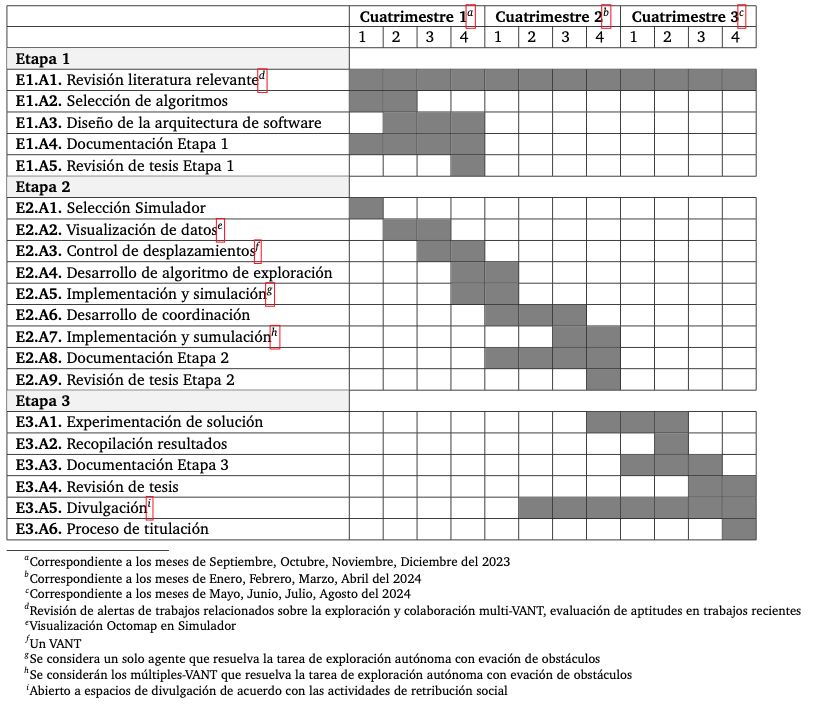
\includegraphics[width=11cm, height=8cm]{cronograma}
  \end{figure}
  
\end{frame}

\section{Estado del Arte}

\begin{frame}{Prueba Video}

  \centering
  \animategraphics[loop, width=10cm]{10}{video-}{0}{46}  
\end{frame}


\begin{frame}
  
  \centering
  \begin{tabular}{ | p{4cm} | p{3cm} | p{3cm} | p{3cm}|}
    \hline
    \hline
    \small REFERENCIA&
    \small MAPA&
    \small Planificador de rutas&
    \small Control de trayectoria\\
    \hline
    \hline
    %--------------------------
    \small \cite{CIESLEWSKI2017}[\citenum{CIESLEWSKI2017}]&
    \small Octomap&
    \small Basado en fronteras&
    \small Control directo de velocidad\\ \hline
    %--------------------------
    \small \cite{USENKO2017}[\citenum{USENKO2017}]&
    \small Cuadr\'{i}cula egoc\'{e}ntrica&
    \small Offline RRT*&
    \small Curvas de Bezier\\ \hline 
    %--------------------------
    \small \cite{MOHTA2017}[\citenum{MOHTA2017}]&
    \small mapa 3D-Local y 2D-Global&
    \small A*&
    \small Prograci\'{o}n cuadr\'{a}tica \\ \hline 
    %--------------------------
    \small \cite{LIN2017}[\citenum{LIN2017}]&
    \small 3D voxel array TSDF&
    \small A*&
    \small Optimizaci\'{o}n cuadr\'{a}tica \\ \hline
    %--------------------------
    \small \cite{PAPACHRISTOS2017}[\citenum{PAPACHRISTOS2017}]&
    \small Octomap&
    \small NBVP&
    \small Control directo de velocidad \\ \hline
    %--------------------------
    \small \cite{OLEYNIKOVA2018}[\citenum{OLEYNIKOVA2018}]&
    \small Voxel Hashing TSDF&
    \small NBVP&
    \small Optimizaci\'{o}n cuadr\'{a}tica \\ \hline
    %--------------------------
    \small \cite{GAO2018}[\citenum{GAO2018}]&
    \small Mapa de cuadr\'{i}cula&
    \small M\'{e}todo de marcha r\'{a}pida&
    \small Optimizaci\'{o}n cuadr\'{a}tica \\ \hline
  \end{tabular}
\end{frame}

\begin{frame}
  
  \centering
  \begin{tabular}{ | p{4cm} | p{3cm} | p{3cm} | p{3cm}|}
    \hline
    \hline
    \small REFERENCIA&
    \small MAPA&
    \small Planificador de rutas&
    \small Control trayectoria\\
    \hline
    \hline
    %--------------------------
    \small \cite{FLORENCE2018}[\citenum{FLORENCE2018}]&
    \small Busqueda basada en visibilidad&
    \small 2D A*&
    \small Control MPC \\ \hline
    %--------------------------
    \small \cite{SELIN2019}[\citenum{SELIN2019}]&
    \small Octomap&
    \small NBVP&
    \small Control directo de velocidad \\ \hline
    %--------------------------
    \small \cite{BUG2019}[\citenum{BUG2019}]&
    \small NA&
    \small SGBA&
    \small Control directo de velocidad \\ \hline
    %--------------------------
    \small \cite{COLLINS2019}[\citenum{COLLINS2019}]&
    \small KD Tree $+$ Mapa en Voxel&
    \small B\'{u}squeda en Grafo&
    \small Movimientos suaves \\ \hline
    %--------------------------
    \small \cite{CINVES2021}[\citenum{CINVES2021}]&
    \small Octree&
    \small RRT&
    \small Basado en contornos \\ \hline
    %--------------------------
    \small \cite{RACER2022}[\citenum{RACER2022}]&
    \small Octomap HGrid&
    \small NBVP&
    \small Control directo de velocidad \\ \hline
    %--------------------------
    %\cite{WESTHEIDER2023}&
    %Mapa de cuadr\'{i}cula&
    %Deep Learning&
    %Control directo de velocidad&
    %\ding{51}\\ \hline
    %--------------------------
    %\cite{BARTOLOMEI2023}&
    %Mapa de cuadr\'{i}cula&
    %NBVP&
    %Control directo de velocidad&
    %\ding{51}\\ \hline
  \end{tabular}
  
  
  
%\begin{figure}
%  \centering
%  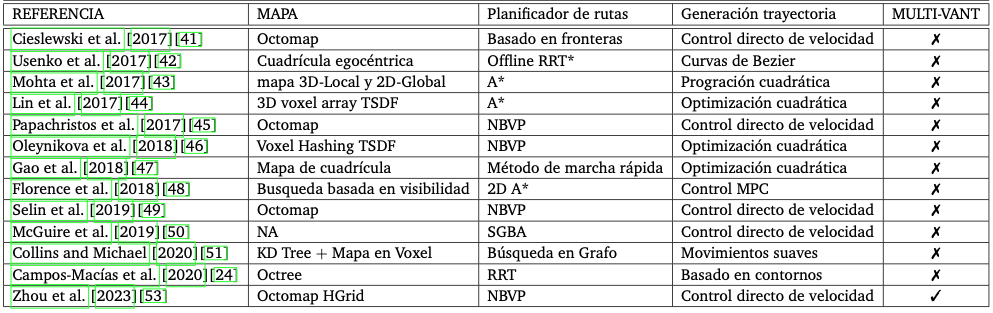
\includegraphics[width=10cm, height=6cm]{estado_del_arte}
%\end{figure}
\end{frame}

\section{Contribuciones o resultados esperados}

\begin{frame}

  \frametitle{Contribuciones o resultados esperados}

  \begin{enumerate}
  \item<1-> Documentación y códigos liberados
    \begin{itemize}
    \item Algoritmo para la exploración multi-VANT
    \item Algoritmo para la planificación de rutas multi-VANT
    \item Protocolo de comunicación y coordinación descentralizados multi-VANT que formaran parte de la arquitectura de software
    \end{itemize}
  \item<2-> Simulación de la solución
  \item<3-> Tesis impresa
  \end{enumerate}
  
\end{frame}

\begin{frame}[allowframebreaks,noframenumbering]
  \frametitle{Bibliografía}
  \bibliographystyle{abbrvnat}
  \bibliography{test}
\end{frame}

\end{document} 
